\documentclass[12pt,a4paper]{report}
\usepackage[english]{babel}
\usepackage[utf8]{inputenc}
\usepackage{color}
\usepackage{amsmath}
\usepackage{mathtools}
\usepackage{graphicx}
\usepackage[export]{adjustbox}
\usepackage{subcaption} %per le figure doppie 
\usepackage{array}
\usepackage{multirow}
\usepackage{tabularborder}
\usepackage{footnote}
\usepackage{caption}
\usepackage{siunitx}
\usepackage{newlfont}
\usepackage{color}
\usepackage{url}
\def\UrlBreaks{\do\/\do-}
\usepackage{breakurl}
\usepackage{hyperref}
\usepackage{enumitem}
\textwidth=450pt\oddsidemargin=0pt
\usepackage{hyperref}
\usepackage{fancyhdr}
\pagestyle{fancy}
\usepackage[Lenny]{fncychap}


\begin{document}




\setlength{\headheight}{15pt}



\begin{titlepage}
%
%
% ONCE YOU ARE FINISHED WITH YOUR CHANGES MODIFY "RED" WITH "BLACK" IN ALL \textcolor COMMENTS
%
%
\begin{center}
{{\Large{\textsc{Alma Mater Studiorum $\cdot$ University of  Bologna}}}} 
\rule[0.1cm]{15.8cm}{0.1mm}
\rule[0.5cm]{15.8cm}{0.6mm}
\\\vspace{3mm}
{\small{\bf School of Science \\
Department of Physics and Astronomy\\
Master Degree in Physics}}
\end{center}

\vspace{23mm}

\begin{center}\textcolor{black}{
%
% INSERT THE TITLE OF YOUR THESIS
%
{\Large{\bf Implementation of an automated pipeline for predicting the response to neo-adjuvant chemo-rediotherapy of colorectal cancer}}
}\end{center}

\vspace{50mm} \par \noindent

\begin{minipage}[t]{0.47\textwidth}
%
% INSERT THE NAME OF THE SUPERVISOR WITH ITS TITLE (DR. OR PROF.)
%
{\large{\bf Supervisor: \vspace{2mm}\\\textcolor{black}{
Prof. Gastone Castellani}\\\\
%
% INSERT THE NAME OF THE CO-SUPERVISOR WITH ITS TITLE (DR. OR PROF.)
%
% IF THERE ARE NO CO-SUPERVISORS REMOVE THE FOLLOWING 5 LINES
%
\textcolor{black}{
\bf Co-supervisor: \vspace{2mm}\\Dr. Nico Curti\\\\}}}
\end{minipage}
%
\hfill
%
\begin{minipage}[t]{0.47\textwidth}\raggedleft \textcolor{black}{
{\large{\bf Submitted by:
\vspace{2mm}\\
%
% INSERT THE NAME OF THE GRADUAND
%
\textcolor{black}{
Giuseppe Filitto}}}
}
\end{minipage}

\vspace{32mm}

\begin{center}
%
% INSERT THE ACADEMIC YEAR
%
Academic Year \textcolor{black}{ 2020/2021}
\end{center}

\end{titlepage}


\clearpage

\begin{abstract}
    Colorectal cancer is a malignant neoplasm of the large intestine resulting from the uncontrolled proliferation of the cells making up the colorectal tract.
    Colorectal cancer isthe second malignant tumor per number of deaths after the lung cancer and the thirdfor number of new cases after the breast and lung cancer. Risk factors for this kind of cancer include colon polyps, long-standing ulcerative colitis, diabetes of type II and also genetic history (HNPCC or Lynch syndrome). In order to get information about diagnosis, therapeutic effect evaluation on colorectal cancer, radiomic analysis can be performed on radiological images through the application of dedicated radiomic algorithms based on segmentation and features extraction. By segmentation we mean the determination of the regions of interest (ROI) in images that are going to be analyzed. In clinical routines, it is carried with manual or semi-manual techniques by radiologists, but this process is time-consuming, highly operator-dependent and subject to operator expertise. By Radiomic features we meant the features coming from radiographic medical images, which can potentially uncover disease characteristics that fail to be appreciated by the naked eye.
    The aim of this project is to implement an automated pipeline based on automatic segmentation of T2 weighted Magnetic Resonance (MR) images exploiting Convolutional Neural Networks in order to predict the response to neo-adjuvant chemo-radiotherapy of colorectal cancer using radiomics features.
\end{abstract}

\clearpage
\thispagestyle{empty}
\begin{flushright}
\null\vspace{\stretch{1}}
\large{\emph{\dots To my family and Nicole}}
\vspace{\stretch{2}}\null
\end{flushright}


\clearpage
\tableofcontents


\chapter{Introduction}

Colorectal cancer is a malignant neoplasm of the large intestine resulting from the uncontrolled proliferation of the cells making up the colorectal tract.
Colorectal cancer is the second malignant tumor per number of deaths after the lung cancer and the third for number of new cases after the breast and lung cancer\cite{cancerstats}.
Among the risk factors for this kind of cancer non hereditary could range from colon polyps to long-standing ulcerative colitis, from Crohn's disease to old age. Also genetic history (HNPCC or Lynch syndrome) and nutritional factors as
diabetes II can increase the probability of develop cancer \cite{tesicoppola}.
Preventive measures for colorectal cancer include physical activity, reducing the consumption of processed meat and alcohol, and avoiding smoking\cite{stats2019}.

\begin{figure}[h!]
	\centering
	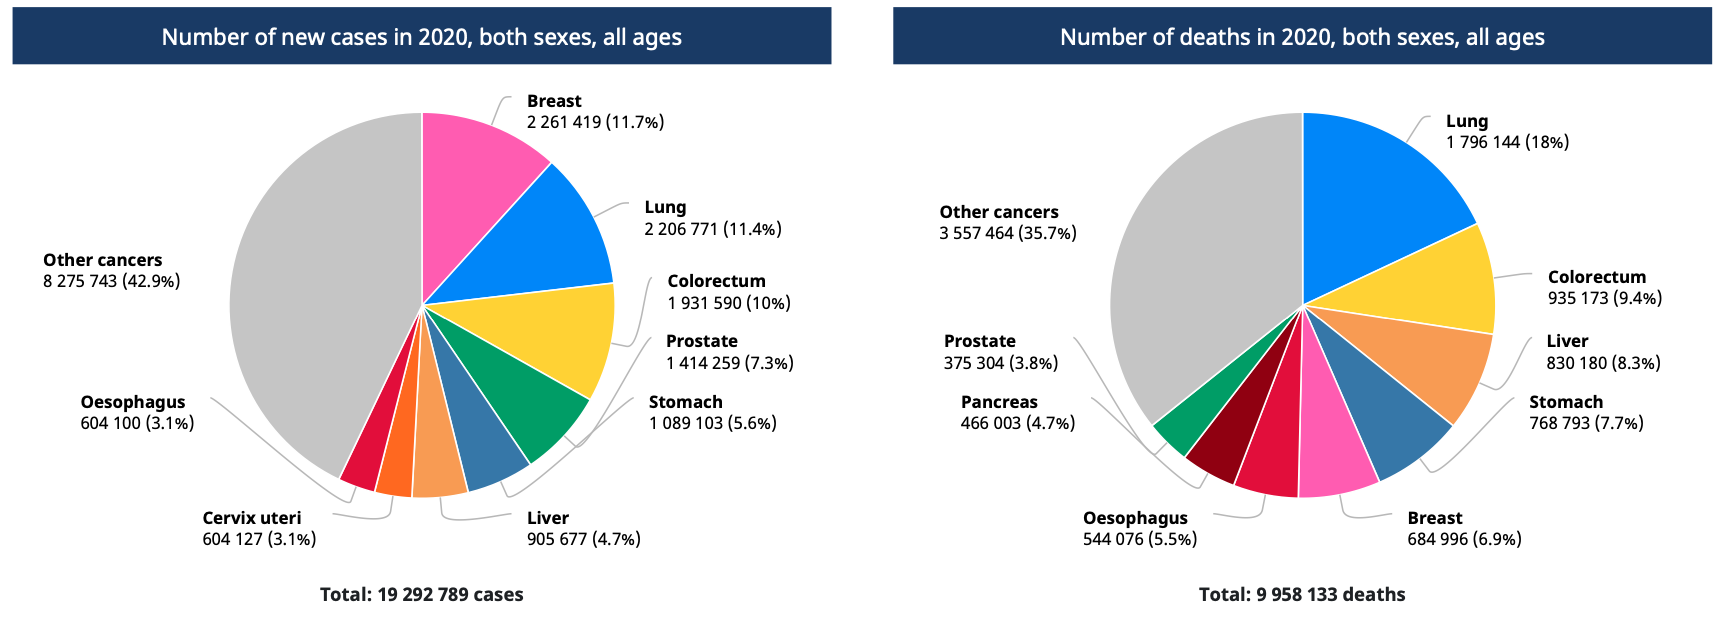
\includegraphics[width=0.8\linewidth]{images/cancerstats.png}
	\caption{World's cancer cases and deaths. From \cite{cancerstats} }
\end{figure}


Screening and diagnosis methods for colorectal cancer can be based on different techniques such as colonoscopy, MRI and CT scans \cite{jovana}. The gold stardand in medical routines is colonoscopy  which is an invasive technique. However, non invasive/destructive methods like Magnetic Resonance and Computed Tomography are also use for tumor staging. In particular MRI, thanks to the high spatial resolution is used for pre-operative predictions and for the evaluation of the neoadjuvant therapy in Colorectal cancer \cite{tesicoppola}.

\begin{figure}[htp]

    \centering
    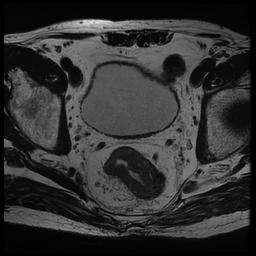
\includegraphics[width=.3\textwidth]{images/T2AX_Alta_8.png}\hfill
    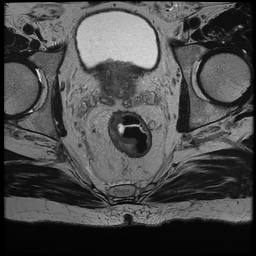
\includegraphics[width=.3\textwidth]{images/T2AX_BO11_5.png}\hfill
    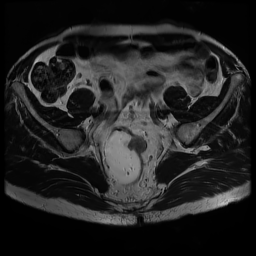
\includegraphics[width=.3\textwidth]{images/T2AX_BO1_9.png}
    
    \caption{T2 weighted axial colorectal cancer MR images. From original dataset}
    \label{trittico}
    
    \end{figure}

In order to get information about diagnosis, therapeutic effect evaluation on colorectal cancer, radiomic analysis can be performed on radiological images through the application of dedicated radiomic algorithms based on segmentation and features extraction. By segmentation we mean the determination of the regions of interest (ROI) in images that are going to be analyzed. In clinical routines, it is carried with manual or semi-manual techniques by radiologists, but this process is time-consuming, highly operator-dependent and subject to operator expertise \cite{jovana, tesicoppola,Trebeschi2017}. Lately, several deep learning techniques in the medical field have been developed exploiting Convolutional Neural Networks (CNN) for medical images segmentation \cite{Trebeschi2017, jovana, tesicoppola}. 

As regard the colorectal cancer segmentation on T2-weighted magnetic resonance, one of the most important study of Trebeschi et al. \cite{Trebeschi2017}, shows how the deep learning approach can perform accurate localization and segmentation of rectal cancer in MR imaging in the majority of patients despite the diffuclt in segmenting a quite important Field-of-View (FOV) as in colorecatal MR images. In Fact, it has been shown how the network performances can vary training the same model with different image annotations or 'labels', taken from different experts, resulting in different Dice-Coefficient (DSC) scores, DSC=0.68 for "reader 1" and DSC=0.70 for "reader 2" respectively. Moreover, not only the labels but also the kind of image, that is to say the kind of tumor can affect the performances of the Networks as resulted in the study of Jovana Panic at al.\cite{panic}, where including cases of mucinous characterized by bright tumoral areas compared to adenocarcinoma, the Dice-Coefficient results in a lower value, in particular DSC=0.58. An overall study about the comparison of different models, in particular different U-Net architectures, for the segmentation of colorectal cancer on T2-weighted magnetic resonance has been carried by Yi-Jie Huang at al.\cite{Huang_2020}, resulting in a Dice-Coefficient score range between 0.52 and 0.75.\\
As regard Radiomic features we meant the features coming from radiographic medical images, which can potentially uncover disease characteristics that fail to be appreciated by the naked eye\cite{wiki:Radiomics}.  
\\
\begin{figure}[htp]
	\centering
	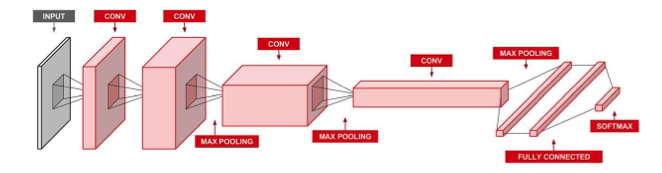
\includegraphics[width=0.9\linewidth]{images/TrebeschiCNN.png}
	\caption{Example of CNN. From \cite{Trebeschi2017} }
\end{figure}

Radiomics features can be divides in different class: shape-size based-features, Haralick's features (Energy, Entropy, Contrast etc...), image voxel descriptors features called GLCM(gray-level co.occurence matrix) and so on. In order to get useful information about the tumor, after segmentation, different approaches have been exploited in literature. For example, in a study of Soomoro at al. \cite{Haraliks}, on T2-weighted magnetic resonance images of colorectal cancer, Haralick's features have been exploited to study the cancer evolution after a segmentation and calssification of tumors depending on the stage malignacy. Another approach consists in clustering all the extracted features after segmentation, in order to get the most relevant ones, as carried in a study of Parmar et al.\cite{featurescluster}.\\
The aim of this project is to implement an automated pipeline based on segmentation and features extraction. As regard the former CNN such as U-Net has been trained from original T2-weighted magnetic resonance images of colorectal cancer dataset, coming from Sant'Orsola Hospital in Bologna, in order to obtain a model to segmented colorectal tumor. As regard the latter, all the possibile features have been extracted for all the patients' examinations and after a reduction analysis the most important ones have been used, integrating clinical data, to predict the response of the patient to the neo-adjuvant chemo-radiotherapy on colorectal cancer. (provvisorio)


\chapter{Segmentation}

Segmentation consists in the determination of the regions of interest (ROI) in images respect to some characteristics such as texture or intensity \cite{Biondi,segmentationreview}. In the medical field, segmetation is performed on medical images and the results can be used for feature extraction to monitor the evolution of a particular disease and/or to evaluate the effects of therapeutical treatements\cite{tesicoppola, Biondi, jovana}. Among the different modalities, the CT-scans and/or MRI-scans can provide anatomical and eventually funcional information about the sunbject anatomy in an non-invasive and non-destructive way. Therefore, segmentation plays a crucial role for medical doctors in identify diseases such as tumors.\\
Segmentation, depending on the technique, can be carried in a manual, semi-manual or automatic way:

\paragraph{Manual segmentation} allows to identify the single pixels/voxels belonging to the tumor tissue with a certain precision and a low margin of physical error. For now it is still the most reliable and precise method but
it is time-consuming, highly operator-dependent and subject to operator expertise\cite{tesicoppola}.

\paragraph{Semi-manual segmentation} is a faster method compared to the manual one and it is based on the traditional image processing methods such as thresholding, clustering and so on. However, despite the time savings it still operator-dependent\cite{tesicoppola}

\paragraph{Automatic segmentation} is possible thanks to development of algorithms and techniques of the Artificial Neural Networks field. In this case, medical references or annotations (labels) and the quantity of images are elements of great importance in order to train the netwotks, in particular for Colorectal cancer, where intrinsic difficulties can arise due to image complexity and the eterogeneity of data\cite{tesicoppola,Trebeschi2017}.


\section{Medical Images}

A medical image is the representation of the anatomical (or functional) structure of the subject of the examination in the form of a pixel/voxel array\cite{Biondi,Larobina}. This discrete representation makes possible processing the data according to the task that is going to be performed (for example increase of the contrast, increase of the brightness etc...). The physical meaning of the data depends on the performed image modality (CT, MRI, SPECT, PET, ...) but in general we can distinguish some characteristics:

\paragraph{Pixel data} refers to the numerical values of the stored pixels depending on the data type (i.e. int, float)\cite{Biondi,Larobina}.

\paragraph{Pixel depth} is the number of bits used to encode the values of each pixel and it is related to the memory space used to store the amount of the encoded information. The most common are [0, 255] for 8-bit image of integers (uint8) and [0, 1] for floats (float32) \cite{Biondi,Larobina}.

\paragraph{Metadata} are informations that describe the image (at least pixel depth, spatial resolution, image matrix dimensions...) stored usually as a header. Medical image metadata can also include information about the patient and the examinaion modality\cite{Biondi,Larobina}.

\paragraph{Photometric interpretation} refers to how the pixel data should be interpreted for the correct image display as a monochrome or color image, for this reason the concept of number of channels must be introduced. Monochrome images have one sample per pixel and no color information stored in the image. In order to encode colours information into pixel we need to multiple samples per pixel and to adopt a color model or color map to specify how to combine the samples\cite{Biondi,Larobina}.

\paragraph{Format} is a standard way to store the information that describe an image. Medical image formats can stadardize the images generated by diagnostic modality (i.e. DICOM) or facilitate the post-processing analysis (i.e. Nifti). As reagrd this project, the images format was the DICOM one. DICOM is the acronym of Digital Imaging and COmmunications in Medicine and it is also a network communications protocols. This file format requires the pixel data not to be separated from to the descriptors of the medical procedures used to the image formation. Finally, DICOM format allows only 2D images so a 3D volume is described by a series of 2D slices \cite{Biondi,Larobina}. Another format which is not properly related to an image is the ROI format, which is related to the region of interest of an image, made as a collection of points represented by x and y coordinates on the image. This file format can be read and made by software like ImageJ/Fiji\cite{Fiji}.


\section{Methods review}

As mentioned before, segmentation methods can be of different type, manual, semi-manual and automatic and at the same time there can be different approaches. For example depending on the requirements of training data, the segmentation methods can be classified in \textit{supervised} and \textit{unsupervised} or depending on the information type, in Pixel clssification methods and \textit{boudary follow} methods\cite{Biondi}.\\
The aim of this section is to give the reader a brief but understandable review on the most common segmentation methods.

\subsection{Thresholding}

Thresholding is a very simple and common approach to segmentation. It consists in binarizing an image into two partitions based on the image intensities (i.e.image histogram)\cite{segmentationreview}. The value which splits the two class is called \textit{threshold} in a way that pixel intensities below this value fall in one class and pixels above falls in the other one as shown in Figure~\ref{threshold}, and for this readon it can be considered a pixel classification technique. Thresholding is often a manual technique based on visual assestment but it can also be performed by automated algorithm like the Otsu one.\\
The main drawback of this techinique consists in the sensitivity to noise and inhomogeneities that make the split of the histogram difficult. However, it is an effective approach for the segmentation of high contrast instensity regions. Moreover, thresholding is usually the first approach used in image segmentation followed by other techniques to improve the results\cite{Biondi}.

\begin{figure}[htp]

    \centering
    \includegraphics[width=.4\textwidth]{images/thresholdexample.png}\hspace{0.5cm}
    \includegraphics[width=.375\textwidth]{images/thresholdhistogram.png}
    
    
    \caption{Example of Histogram Thresholding on a T2 weighted axial colorectal cancer MR images obtained using Fiji software\cite{Fiji}.}
    \label{threshold}
    
    \end{figure}

\subsection{Region growing}

Region growing approach is a segmentation method based on the selection of initial seed points (ususally manually selected)\cite{wiki:regiongrowing}. This approach examines neighboring pixels of initial seed points and according to predefined criteria based on intensity and or edges, the pixel are added to the region. Then, the continuity of the rule application, makes the region growing\cite{Biondi}.\\
The main drawbacks of this method are related to the fact that:

\begin{itemize}[label={\textbf{*}} ]
    \item It is a local method without a gloab view of the problem
    \item Like the thresholding it is sentitve to noise
    \item for each region a seed must be planted
\end{itemize}

However, there are some algorithms like the split and merge one that don't require a seed. Indeed, acting recursively, checking the pixel intensity homogeneity the region can be splitted into sub regions or merged with adjacent regions with similar intensities\cite{wiki:regiongrowing, Biondi}.

\subsection{Clustering}

Clustering is a non surpevised approach that is able to classify pixels without a training dataset. The main task of the clustering is to group a set of objects so that objects in the same group (called a cluster) are more similar (in some sense) to each other than to those in other groups (clusters).The notion of  "cluster" cannot be precisely defined, that is why there are many clustering algorithms. Clustering can be performed also for tasks different from segmentaion like features reduction. Among the different cluster models we can found\cite{wiki:clustering}:

\begin{itemize}[label={\textbf{*}} ]
    \item Centroid models: for example, the k-means algorithm which represents each cluster by a single mean vector.
    \item Distribution models: clusters are modeled using statistical distributions, such as multivariate normal distributions.
    \item Connectivity models: for example, hierarchical clustering that builds models based on distance connectivity.
    \item Density models: for example, DBSCAN that defines clusters as connected dense regions in the data space.
    \item Neural models: for example, unsupervised neural network.
\end{itemize}


\subsection{U-Net}

The U-net is a convolutional network architecture for fast and precise segmentation of images especially in the biomedical field\cite{unet}.
A convolutional neural network (CNN) is a class of deep neural network, most commonly applied to analyze visual imagery\cite{wiki:cnn}. One of the main advantage of the U-net is the ability of dealing with small dataset. The name U-net refers to the U shape of the network architecture. As a matter of fact, the whole structure is divided into two main parts as shown in Figure~\ref{unet}:
\begin{itemize}[label=\textbf{*}]
    \item Encoder: or contraction path is a sequence of convolutional and pooling layers whit the aim of extracting features and redure dimensionality
    \item Decoder: or expansion path is a sequence of transpose convolutional and up-sampling layers aimed to reconstract the segmentation map after the application of an activation function such as \textit{sigmoid} or \textit{softmax}
\end{itemize}
 A convolutional layer can be defined as a sequence of convolutional operations followed by some optional operation like batchnormalization and/or dropout and an activation function such as \textit{ReLu}. Similiraly, a transpose convolutional layer can be defined as a sequence of transpose convolutions. This kind of layer is applied from the very last convolutional layer application and then after the concatenation of the de-convoluted layer with the relative convoluted layer as showed by the grey arrows in Figure~\ref{unet}.


\begin{figure}[h!]
	\centering
	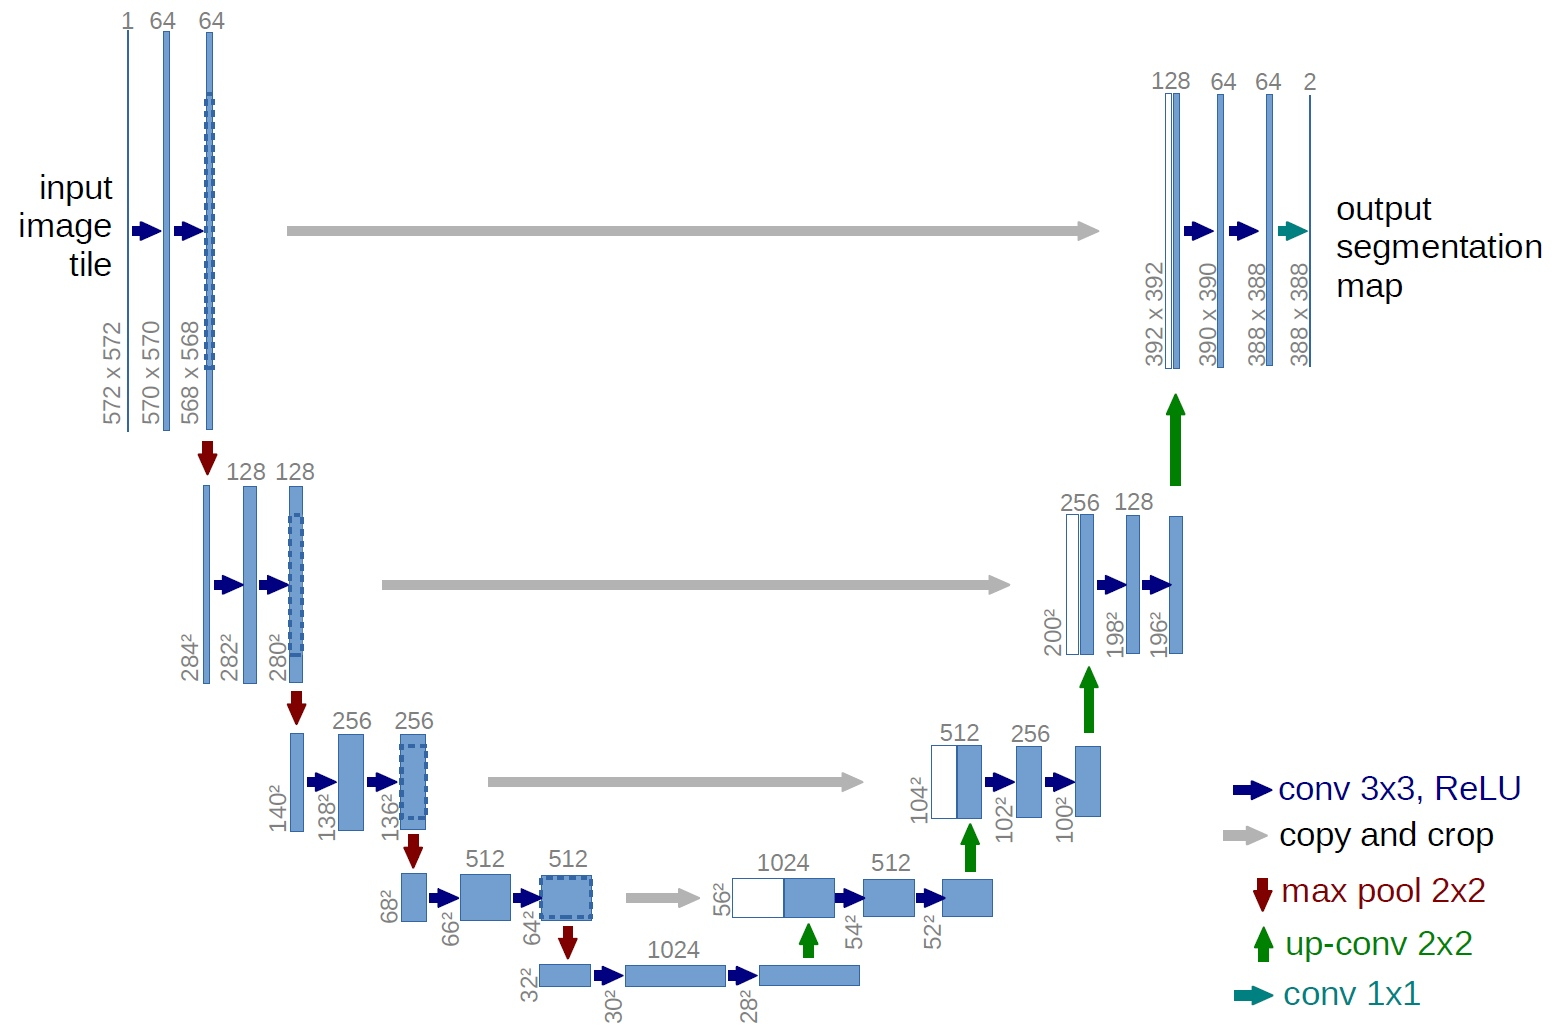
\includegraphics[width=0.8\linewidth]{images/U-Net arch.jpeg}
	\caption{Original U-Net architecture. From \cite{unet} }\label{unet}
\end{figure}

\subsubsection{Backbone}

The backbone refers to the network which extracts the feature map upon which the rest of the network is based\cite{cnnbackbones}. A backbone can be made also of different network architecture itself. For example, we can define a backbone like the ensamble of convolutional layers or define our own architecture. The advantage of using a backbone is to improve the performances of the features extraction and so of the whole network\cite{cnnbackbones}. An overview of the most common backbones will be given in the following paragraphs.

\paragraph{VGG16} is a convolutional neural network model proposed by K. Simonyan and A. Zisserman from the University of Oxford in \textit{"Very Deep Convolutional Networks for Large-Scale Image Recognition"}\cite{vgg16}.
The pecularity of VGG16 is a not so high number of hyper-parameter and many convolution layers as shown in Figure~\ref{vgg16}.The 16 in VGG16 refers to it has 16 layers that have weights, but other versions with more layers, such as VGG19, exist.

\begin{figure}[h!]
	\centering
	\includegraphics[width=0.6\linewidth]{images/vgg16.png}
	\caption{VGG16 architecture. From \cite{url:vgg16} }\label{vgg16}
\end{figure}

\paragraph{MobileNet} is based on depthwise separable convolutions which is a form of factorized convolutions which factorize a standard convolution into a depthwise convolution and a 1 × 1 convolution called a pointwise convolution, in  order to reduce computational cost\cite{mobilenet}.

\begin{figure}[h!]

    \centering
    \includegraphics[width=.3\textwidth]{images/conv.png}
    \includegraphics[width=.3\textwidth]{images/deptwiseconv.png}
    
    \caption{Convolutional layers vs Depthwise convolutional layers. From \cite{mobilenet}}
    \label{mobilenet}
    
    \end{figure}

\paragraph{ResNet} is a residual neural network faimily characterized by the so called, residual blocks, based on the \textit{Identity shortcut connection}, as shown in Figure~\ref{resnet}, which skips one or more than one layers\cite{resnet}. Based on ResNet, similiar architecture with different residual blocks were developed, such as ResNeXt.

\begin{figure}[h!]
	\centering
	\includegraphics[width=0.5\linewidth]{images/residualblock.png}
	\caption{Residual block. From \cite{resnet} }\label{resnet}
\end{figure}

\paragraph{EfficientNet} is a family of models based on scaling\cite{efficientnet}. Generally, it is done to improve the model performances and efficiency on a certain task and, as shown in Figure~\ref{efficientnet}, it can be of different kind. Scaling a network by depth is the most common way of scaling. Depth can be scaled up as well as scaled down by adding/removing layers respectively\cite{url:efficientnet}. According the model's architecture  settings, EfficientNet models are named EfficientNet-B0, EfficientNet-B1 and so on.

\begin{figure}[h!]
	\centering
	\includegraphics[width=0.9\linewidth]{images/scaling.png}
	\caption{Example of model scaling. From \cite{efficientnet} }\label{efficientnet}
\end{figure}


\chapter{Radiomics}

Radiomics is a method that, using data-characterisation algorithms, from  medical images extracts a large number of features which
have the potential to uncover disease characteristics that fail to be appreciated by the naked eye\cite{wiki:Radiomics}. The main objective of radiomics is to assist the subjective interpretation of the doctor with an objective prediction of all those data invisible to the radiologist, transforming medical images into data, defined as \textit{biomarkers}, thus allowing to provide a complete quantification of the tumor phenotype\cite{tesicoppola}. In the new era of precision medicine, radiomics is an emerging translational research field that aims to find associations between qualitative and quantitative information extracted from clinical images and clinical data to support decision making process. Thanks to this data, it is possible to create a personalized therapy for each patient according to his characteristics. Radiomics analysis can be performed in tumor regions, metastatic lesions and normal tissues\cite{tesicoppola}.

\section{Features}

Radiomic features can be divided into five groups\cite{wiki:Radiomics, tesicoppola}:

\begin{itemize}[label=\textbf{*}]
    \item size and shape based–features like descriptors of the image intensity histogram, gray-level co-occurrence matrix (GLCM);
    \item run length matrix (RLM);
    \item size zone matrix (SZM);
    \item neighborhood gray tone difference matrix (NGTDM) derived textures, textures extracted from filtered images;
    \item fractal features.
\end{itemize}

\section{Possible purposes of radiomics}

The possible applications of radiomics are based on a very wide range, from the prediction of clinical outcomes to the oncological diagnosis. In particular, thanks to the development of Artificial Intelligence (AI) there might not be needed to resort to biopsy, which is not only invasive but requires a well-trained doctor and important technical times. In addition, AI might be able to support the medical doctor in formulating and validating a diagnosis with more data, thus giving a (virtual) second opinion\cite{tesicoppola}.\\
In this section, among the several possible purposes, a brief overview of some of them will be given.


\subsection{Prediction of clinical outcomes}

Radiomic features may be useful for predicting patient survival and describing intratumoral heterogeneity as demonstrated in a study by Aerts et al \cite{Aerts}. Many other studies have also shown that radiomic characteristics are better at predicting response to treatment than conventional measures such as tumor volume and diameter, and maximal uptake of the FDG radiotracer in positron emission tomography (PET) imaging. More, the usefulness of radiomics for predicting the immunotherapy response of patients with non-small cell lung cancer (NSCLC) using pretreatment CT and PET-CT images has been demonstrated by other studies\cite{tesicoppola}.

\subsection{Prediction of metastases}

Radiomic features can also predict the metastatic potential of tumors. 
For example, many radiomic features were identified as predictors of distant metastasis of lung adenocarcinoma in a study by Coroller et al. \cite{Coroller}. They concluded that radiomic features may be useful in identifying patients at high risk of developing distant metastases, guiding doctors in choosing the most effective treatment for individual patients\cite{tesicoppola}.


\subsection{Genetic evaluation of cancer}

The biological mechanisms of colorectal cancer were studied for the construction of different imaging models. In particular, It has been showed that radiomic features can be associated with some biological genes\cite{tesicoppola}. This type of study was also carried out at the brain level. In fact, in a study on T2-weighted MR images, various mutations of glioblastoma (GBM), have shown to be significantly predictable from texture and shape based radiomic features\cite{glioblastoma}.

\subsection{Prognosis formulation}

Since the aggressiveness of a tumor even at the same stage can vary depending on the patient, determinig it is essential to allow the best possible management for the patient. Studies have shown that image-based markers could provide staging and biomarkers information to improve the prgnosis\cite{tesicoppola}.


\subsection{Prediction of physiological events}

Another possible application of radiomics analysis is the prediction of physiological events. Indeed, radiomics can be applied for the characterization and investigation of complex physiological events such as brain activity, which is usually studied with specific imaging techniques such as functional magnetic resonance "fMRI". Raw fMRI images can be subjected to radiomic analysis which can subsequently be correlated with the brain activity\cite{tesicoppola}.


\chapter{Pipeline}

The aim of this project is to implement an automated pipeline based on automatic segmentation of T2 weighted Magnetic Resonance (MR) images exploiting Convolutional Neural Networks in order to predict the response to neo-adjuvant chemo-radiotherapy of colorectal cancer using radiomics features. 

\section{Description}

The pipeline workflow is made by different steps, each one performing a different task. The aim of this section is describe how each step of the pipeline is achieved. As reagrd the implementation, it will be described in the solllowing section.


\subsection{Pre-processing}

\subsection{Segmentation}

\subsection{Features Extraction}

\subsection{Predictions}

da valutare appena sarà completato il progetto

\section{Implementation}


\paragraph{Pre-processing}
\paragraph{Segmentation}
\paragraph{Features Extraction}
\paragraph{Predictions}



\chapter{Results}

\section{Dataset description}

The data come from the surgical database of the Sant' Orsola Polyclinic, containing patients with colorectal cancer undergoing neo-adjuvant radio-chemotherapy, from January 2018 to the end of December 2019. In our case, 48 patients were considered.


\section{Segmentation}

\subsection{CNN Training}
\subsection{Segmentation outcomes}

\section{Features Extraction}

\section{Predictions}


\chapter{Conclusions}


\clearpage

\bibliographystyle{unsrturl}
\bibliography{bibliography}



\end{document}